\section{Decentralizovaná optimalizácia}
\label{se:DecentralizovanaOptimalizacia}
Zvyčajne, pri všeobecnej optimalizačnej úlohe, si ako prvé zadefinujeme účelovú funkciu, určíme si začiatočné podmienky a ohraničenia potom zvolíme vhodnú optimalizačnú metódu pre nájdenie optima. Takto formulovanú optimalizáciu nazývame centralizovaná optimalizácia, kde sa všetky premenné nachádzajú pod jedným problémom a výsledkom je centralizované riešenie:
\begin{subequations}
	\begin{align}
		\displaystyle \min_{x} \hspace{0.5cm} & 
		f(x),\\
		\textrm{v.n.} \hspace{0.5cm} & Lx = v.
	\end{align}
\end{subequations}
V tejto práci ale využijeme takzvanú decentralizáciu optimalizačného problému. Optimalizačnú úlohu si rozložíme na viacero častí $ f(x) = g(z) + h(y)$ a každú riešime samostatne. Výsledkom bude viacero decentralizovaných riešení. Rovnice (2.9) si rozdelíme vzhľadom k jednotlivým premenným a budú mať nasledovný tvar:
\begin{subequations}
	\begin{align}
		\displaystyle \min_{} \hspace{0.5cm} & 
		g(z) + h(y),\\
		\textrm{v.n.} \hspace{0.5cm} & L_{1}z = v_1,\\
		& L_{2}y = v_2.
	\end{align}
\end{subequations}
Takéto rozloženie účelovej funkcie na viac častí umožňuje zjednodušenie optimalizačnej úlohy a pri riešení náročných optimalizácií môže výrazne skrátiť čas výpočtu.
\begin{figure}[H]
	\centering
	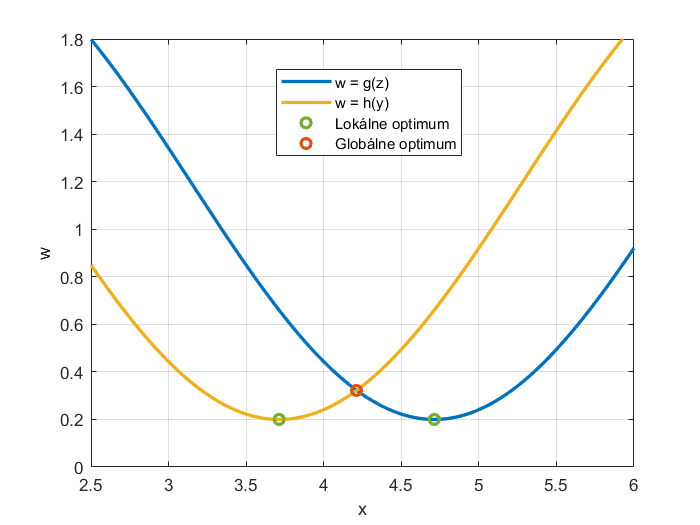
\includegraphics[width=11cm,height=8cm]{images/Global_Local_ADM}
	\caption{Porovnanie globálneho a lokálneho riešenia}
\end{figure}
Jedným z problémov, ktorý môže nastať pri decentralizovanej optimalizácií je, že jednotlivé decentrálne riešenia môžu uviaznuť vo svojich lokálnych optimách (Obr. 2.2). Teda cieľom decentralizovanej optimalizácie bude aj, aby jednotlivé riešenia nekonvergovali do lokálneho, ale do jedného globálneho optima. 
\section{ADMM}
\label{subse:ADMM}
ADMM je skratka z anglického názvu (Alternating Direction Method of Multipliers). Pomocou tejto metódy vieme riešiť decentralizovaný optimalizačný problém.
Formulácia optimalizačného problému pre ADMM je v nasledovnom tvare:
\begin{subequations}
	\begin{align}
		\displaystyle \min_{y,z} \hspace{0.5cm} & 
		g(z) + h(y),\\
		\textrm{v.n.} \hspace{0.5cm} & H_{1}z + H_{2}y = b,
	\end{align}
\end{subequations}
kde $y$ a $z$ sú optimalizované premenné, ktoré sú definované nasledovne $y \in {\rm I\!R}^n $, $ z\in {\rm I\!R}^m$. Rovnica (2.11b) predstavuje novú podmienku, ktorá prepája decentralizované premenné, matica $H_{1}$, $H_{2}$ a vektor $b$ sú skonštruované tak, aby podmienky boli vhodné pre všetky prípady, ich rozmery sú $H_{1} \in {\rm I\!R}^{p \times n}$, $H_{2} \in {\rm I\!R}^{p \times m}$ a teda vo výsledku je vektor $b \in {\rm I\!R}^p $. 

Ako môžeme vidieť, rozdiel medzi decentralizovaným a centralizovaným optimalizačným problémom je, že sme rozdelili optimalizované premenné, spolu s účelovou funkciou, ktorá musí umožňovať takéto rozdelenie premenných. S takýmto rozdelením nám zároveň pribudla nová podmienka do optimalizačného problému, ktorá prepája rozdelenú funkciu. Táto podmienka sa nazýva duálna funkcia. 
Ďalej môžeme pokračovať tak, že túto novú podmienku pridáme do optimalizačného problému pomocou Lagrangianovej metódy a vytvoríme rozšírenú Lagrangianovú funkciu:
\begin{equation}
	\mathcal{L}_{\rho} = g(z) + h(y) + \lambda^{T}\left(  H_{1}z + H_{2}y - b \right) + \frac{\rho}{2} \norm{H_{1}z + H_{2}y - b}_{2}^{2}.
\end{equation}
Rozšírenie Lagrangianovej funkcie predstavuje posledný člen $\frac{\rho}{2} \norm{H_{1}z + H_{2}y - b}_{2}^{2}$ a zabezpečuje, aby bola funkcia spojite diferencovateľná a zároveň pomáha konvergencii. Pridaním tohoto člen neovplyvníme hodnotu optima, keďže je v optime nulové. Takto definovanú úlohu vieme riešiť separátnym prístupom k jednotlivým premenným Lagrangianovej funkcie $\mathcal{L}_{\rho} \left(z,y,\lambda \right)$:
\label{math:ADMM_iteracie}
\begin{subequations}
	\begin{align}
		&z^{(i+1)} = \argmin_{z} \mathcal{L}_{\rho} \left(z,y^{(i)},\lambda^{(i)} \right),\\
		&y^{(i+1)} = \argmin_{y} \mathcal{L}_{\rho} \left(z^{(i)},y,\lambda^{(i)} \right),\\
		&\lambda^{(i+1)} = \lambda^{(i)} + \rho\left( H_{1}z^{(i+1)} + H_{2}y^{(i+1)} - b \right),
	\end{align}
\end{subequations}
kde $\rho > 1$ a $i$ hovorí o tom v akej iterácií sa nachádzame. Táto iteračná metóda prebieha v takzvanom duálnom framworku, ktorý sa skladá z primárneho problému (minimalizácia $z$, minimalizácie $y$) a aktualizácie duálneho problému $\lambda$. V poslednom vzťahu, kde sa aktualizuje duálna premenná, je aplikovaný podobný postup ako v numerickej gradientovej metóde, ale vykoná sa iba raz, $\rho$ tu predstavuje dĺžku kroku. Funkcia tohoto duálneho problému je konkávna, a teda sa ľahko maximalizuje, čo nespôsobuje ťažkosti, ak náš primárny problém je konvexný. Ak primárny problém spĺňa konvexnosť tak jeho minimum korešponduje s maximom duálneho problému. Preto neoptimalizujeme v smere poklesu (ako tomu je pri minimalizácii v gradientovej metóde), ale hýbeme sa v smere rastu\cite{bib1}. 
\label{subse:ADMM2}

Postup pri iterácií v ADMM:
\begin{description}
	\item[Krok 1:] {Paralelne vyriešime minimalizáciu Lagrangianovej funkcie vzhľadom k všetkým predikčným horizontom, \hyperref[math:ADMM_iteracie]{rovnice (2.13a,2.13b)}.}
	\item[Krok 2:] {Aktualizujeme duálny parameter $\lambda$ s novými hodnotami, \hyperref[math:ADMM_iteracie]{rovnica (2.13c)}.}
	\item[Krok 3:] {Opakujeme od kroku 1, až kým skonvergujeme do globálneho minima (narazíme na zastavovacie kritérium).}
\end{description}

